\documentclass[12pt]{article}

\usepackage{graphicx}
\usepackage[margin=1.0in]{geometry}
\usepackage{amsmath}
\usepackage{cases}
\usepackage{amsfonts}
\usepackage{amssymb}
\usepackage{grffile}
\usepackage{setspace}

\setlength\parindent{0pt}

\author{Xiaohui Chen \\EID: xc2388}
\title{M 362K Post-Class Homework 3}

\begin{document}
\maketitle
\begin{spacing}{2.0}

\section*{2-2}
\subsection*{(a)}
$A\cap B=\{1,2\}$

\subsection*{(b)}
$B'=\{\pi,water\}$

$\therefore N(B')=2$

\subsection*{(c)}
$A\cup B=\{1,2,\pi,Jamaal,gum\}$

$\therefore (A\cup B)'=\{water\}$

\section*{2-7}
We let the number of king-size matresses sold to be x, queen-size to be y and twin-size to be z

According to the question, we get: $\frac{1}{4}y=x+z$ and $3x=z$

By arranging the formulas, we get $x=\frac{z}{3}$ and $y=\frac{16}{3}z$

According to the axioms of probability theory, $Pr(king or queen)=1-Pr(twin)=1-\frac{z}{\frac{z}{3}+ \frac{16z}{3}+z}= 1-0.15= 0.85$

Therefore the probability that the next mattress sold is wither king or queen-size is 0.85, which is (D)

\section*{2-14}
Since $N(U)=20$, $N(A)=N(U)-N(A')=6$ and $N(B)=N(U)-N(B')=10$

Using the inclusion-exclusion principle, $N(A\cap B)= N(A)+N(B)-N(A\cup B)=6+10-12=4$

\section*{2-19}
Using the inclusion-exclusion principle $Pr(automobile\cup house)=Pr(automobile)+ Pr(house)+ Pr(automobile\cap house)= 0.6+0.3-0.2= 0.7$

$\therefore Pr(automobile or house, not both)= Pr(automobile\cup house) - Pr(automobile\cap house)= 0.7-0.2=0.5$

The answer is (B)

\section*{2-21}
Using the inclusion-exclusion principle, we get:

$Pr(gymnastics\cup baseball \cup soccer)= Pr(gymnastics)+ Pr(baseball) + Pr(soccer)- Pr(gymnastics\cap baseball)- Pr(gymnastics \cap soccer) - Pr(baseball\cap soccer) + Pr(gymnastics\cap baseball \cap soccer)= 0.28+0.29+0.19-0.14-0.12-0.1+0.08= 0.48$

$Pr(watch none)=1-Pr(gymnastics\cup baseball \cup soccer)= 1-0.48=52\%$

Therefore, the answer is (D)

\section*{2-23}
$Pr(A\cup B)=Pr(A)+Pr(B)-Pr(A\cap B)$

$Pr(A\cup B')=Pr(A)+Pr(B)-Pr(A\cap B')$

$Pr(A\cup B)+ Pr(A\cup B')=Pr(A)+Pr(B)-Pr(A\cap B)+ Pr(A)+Pr(B)-Pr(A\cap B')=2Pr(A)+(Pr(B)+Pr(B'))-(Pr(A\cap B)+Pr(A\cap B'))= 2Pr(A)+1-Pr(A)=Pr(A)+1=1.6$

$\therefore Pr(A)=0.6$

The answer is (D)

\section*{2-25}
\begin{figure}
  \centering
  % Requires \usepackage{graphicx}
  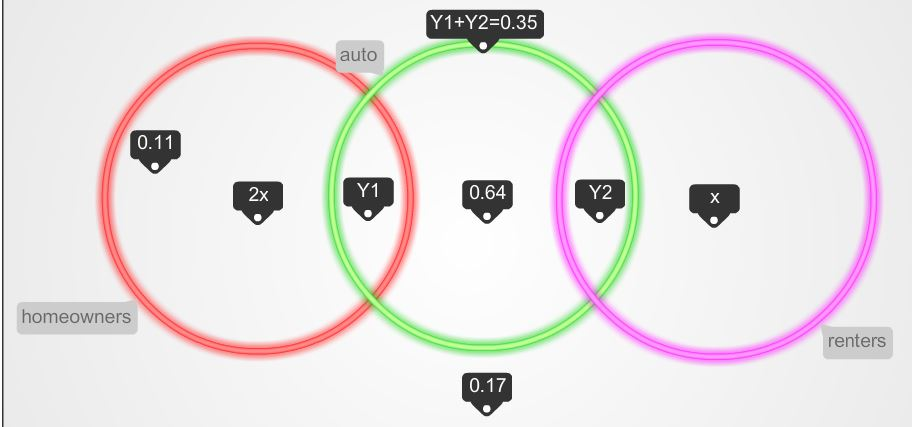
\includegraphics[width=5in]{venn}\\
  \caption{The Venn Diagram of 2-25}\label{venn}
\end{figure}

The Venn diagram is shown in Figure \ref{venn}. The diagram is made according to the information given in the question

We can know that $Pr(renters only)=1-0.17-0.11-0.64=0.08$

Therefore, we can know that 2*(0.08+Y2)=0.11+Y1

Since $Y1+Y2=0.35$, we can know that $Pr(auto\cap renters)= 0.1=10\%$

The answer is (B)

\end{spacing}
\end{document}